%% ------------------------------------------------------------------------- %%
\chapter{Conceitos básicos}
\label{cap:conceitos}

Neste capítulo apresentaremos conceitos que são base para esta pesquisa.
Os conceitos apresentados serão sobre serviços web e suas composições, 
implantação de sistemas, e por fim os desafios particulares da implantação
de sistemas de grande escala.

%pra intro?
%Em nosso trabalho, estudaremos como as soluções de implantação automatizada
%apoiadas por middleware facilitam o apoio à implantação de sistemas de grande escala.

\section{Serviços web}
\label{sec:servicos}

Serviços são entidades autônomas e independentes de plataforma, que podem ser descritas, publicadas, encontradas e compostas~\cite{Papazoglou2007State}. O conceito de serviço é oriundo do conceito de \emph{componentes}, que foram idealizados para que sistemas fossem construídos com ``blocos'' fornecidos por terceiros~\cite{McIlroy1968MassProduced}. Esses blocos teriam interfaces bem definidas e, com isso, seriam conectáveis entre si, sem que o desenvolvedor precisasse entender sobre a implementação desses blocos. Szyperski~\cite{Szyperski2003Component} define componente como uma unidade de composição, possuindo uma especificação de interface contratual e declaração explícita de suas dependências. Dessa forma, um serviço também é considerado um componente, porém com algumas características peculiares, como ser acessível pela rede e expor operações relacionadas a funcionalidades do negócio~\cite{Hewitt2009JavaSOA}. 

%Um exemplo bem conhecido de padronização de sistemas baseados em componentes é o Common Object Request Broker Architecture (CORBA). A especificação CORBA~\cite{CORBA1995} define objeto como uma ``entidade encapsulada e identificável que fornece um ou mais serviços que podem ser requisitados por um cliente'', o que corresponde ao conceito de componente. Ainda na especificação CORBA, uma interface é definida como uma ``descrição do conjunto de possíveis operações que um cliente pode requisitar para um objeto por essa interface''. Uma interface de um componente CORBA é concretamente descrita utilizando-se a Interface Description Language (IDL). \fabio{Livro básico de componentes: QA754.4 S999c; Procurar CORBA componente model}

Como muitos dos trabalhos sobre implantação de componentes, a serem apresentados no Capítulo~\ref{cap:relacionados}, são diretamente aplicáveis na implantação de serviços, trataremos os termos ``componente'' e ``serviço'' como sinônimos, assim como faz Fowler~\cite{Fowler2004Inversion}. Neste trabalho utilizaremos também os termos ``serviço'' e ``serviço web'' de forma equivalentes, assim como feito por outros autores~\cite{Watson2006Dynasoar}. Daremos preferência ao termo ``serviço web'' para evitar os significados mais gerais que a palavra ``serviço'' pode assumir. Exceção poderá haver quando estivermos descrevendo trabalhos de terceiros que utilizam o termo ``serviço'' com algum significado mais amplo que o de ``serviço web''. Um ponto de acesso (\textit{endpoint}) de um serviço web é uma entidade referenciável para a qual se envia mensagens construídas de acordo com a especificação do serviço~\cite{W3C2004Addressing}. Um ponto de acesso é referenciado por uma URI (\emph{Uniform Resource Identifier}) que possibilita o acesso a esse serviço pela Internet. Assim como Smith e Murray~\cite{Smith2010Evolution}, também utilizaremos a palavra serviço como simplificação para o ponto de acesso do serviço. 

As tecnologias mais utilizadas atualmente para a implementação de serviços são \emph{SOAP} e \emph{REST}. Os serviços SOAP utilizam um conjunto específico de protocolos definidos pela W3C. As mensagens trocadas pelos serviços SOAP possuem uma estrutura (envelope) encapsulada em mensagens HTTP, protocolo utilizado como um meio de transporte. Já os serviços REST utilizam o HTTP como protocolo de aplicação, utilizando assim diretamente os princípios arquiteturais que são utilizados para explicar a alta escalabilidade do protocolo HTTP e da própria World Wide Web~\cite{Pautasso2008Restful}. 

O W3C chama os serviços SOAP como ``serviços web'', fornecendo a seguinte definição: ``serviços web possibilitam a comunicação interoperável entre máquinas pela rede, utilizando padrões abertos para a troca de mensagens e descrição da interface dos serviços~\cite{W3C2004WS}''. Na prática, a única diferença dos serviços REST para essa definição é que em REST não se exige a descrição do serviço em linguagem legível por máquina, embora isso seja possível com a WADL~\cite{WADL2006}. Além disso, nessa definição da W3C também poderiam ser enquadradas outras tecnologias como CORBA~\cite{CORBA1995}. 

Serviços SOAP descrevem suas interfaces com a Web Service Descritption Language (WSDL), interagem entre si pela troca de mensagens SOAP e são publicados e descobertos em repositórios UDDI. Uma interface de um serviço web descrita em WSDL é um arquivo XML com uma estrutura padronizada, o que possibilita a outros sistemas analisarem as possíveis formas de interação com esse serviço. Mensagens SOAP também são estruturadas em XML, sendo normalmente enviadas no corpo de requisições e respostas HTTP. O envelope de uma mensagem SOAP codifica a requisição ou resposta à operação de um serviço web, descrevendo também os tipos de dados e valores envolvidos na operação. 

Além dos padrões mencionados (WSDL, SOAP, UDDI), há vários outros padrões que formam o conjunto chamado de WS-*, que inclui especificações para a realização de transações entre serviços, troca de endereços de serviços, composição de processos de negócios e muitos outros. O uso desse conjunto de padrões de forma integrada relaciona-se com a criação de Arquiteturas Orientadas a Serviços (SOA). De acordo com Papazoglou~\cite{Papazoglou2007State}, SOA é uma forma de projetar sistemas que forneçam serviços com interfaces publicadas que possam ser descobertas, de modo que funcionalidades da aplicação sejam reutilizáveis como serviços por outras aplicações ou serviços em um ambiente distribuído. 

Serviços REST utilizam como \emph{interface uniforme} os verbos do protocolo HTTP (GET, POST, PUT e DELETE) e comunicam-se fazendo uso do protocolo HTTP como protocolo de aplicação para a troca de \emph{representações} de \emph{recursos}, que são identificados por URIs. Recursos são entidades do domínio do negócio que são de interesse dos clientes, e suas representações não estão presas a um formato de troca de mensagens, pois a cada mensagem o formato é descrito por um tipo MIME (ex: xml, json, png, txt). Em REST, também não existe a noção de registro de serviços, pois a identificação de recursos por URIs e o uso de hyperlinks nas próprias mensagens REST possibilitam que os serviços necessários para a aplicação sejam encontrados~\cite{Pautasso2008Restful}.

Ainda segundo Pautasso~\cite{Pautasso2008Restful}, serviços REST são considerados ``mais simples'' do que serviços web porque fazem uso de padrões já bem estabelecidos, como HTTP, XML, URI e MIME, para os quais já existe uma ampla infraestrutura implantada. Um exemplo disso, é que é possível testar alguns serviços REST apenas com um navegador comum. Parte da escalabilidade atribuída a serviços REST também vem desse uso de padrões bem estabelecidos, pois os \emph{caches} implementados pelos servidores web tornam-se automaticamente caches para serviços REST~\cite{Tong2010CXF}.

Apesar das vantagens apresentadas dos serviços REST, serviços que utilizam a tecnologia WS-* ainda são mais propensos a uma série de manipulações automatizadas que se tornam mais difíceis nos serviços REST, como por exemplo a geração automatizada de clientes para uma dada linguagem de programação. Isso se deve principalmente pelo alto nível de padronização da tecnologia WS-* e pela existência de interfaces bem definidas e processáveis por software (WSDL). 

\section{Composições de serviços web}
\label{sec:composicoes}

Serviços são compostos para implementar processos de negócios mais sofisticados~\cite{Papazoglou2007State}. Processos de negócio são sequências bem definidas de passos computacionais executados de uma maneira coordenada~\cite{Alonso2002Atomicity}. A principal tecnologia para a implementação de processos de negócios são os sistemas de gerenciamento de workflow~\cite{Agostini2000Improving}. Um workflow é a automação, total ou parcial, de um processo de negócio, no qual documentos, informações ou tarefas são passados de um participante (humano ou não) para outros, de acordo com um conjunto de regras de procedimento~\cite{WorkflowCoalition1999}. Segundo Casati et al.~\cite{Casati1998Workflow}, workflows são compostos de \emph{tarefas}, unidades de trabalho a serem desempenhadas por agentes humanos ou automatizados e \emph{conectores}, que definem a ordem em que as tarefas devem ser executadas, o que também é denominado \emph{fluxo de controle}. Sincronizações de execuções concorrentes também são especificadas por controladores chamados ``joins'' e ``forks''. Quando uma tarefa é desempenhada por um agente automatizado, o gerenciador de workflow normalmente realiza a invocação de um serviço web, que é esse agente automatizado que participa do processo de negócio. Um exemplo de linguagem para a criação de processo de negócio a partir da composição de serviços web é a WS-BPEL~\cite{BPEL2007}.

O modelo de composição de serviços web no qual temos um coordenador central que coordenada o fluxo de controle da composição é denominado \emph{orquestração}~\cite{Nanda2004Decentralizing}. O coordenador central é chamado de \emph{orquestrador}. No caso em que processos de negócios são executados por sistemas gerenciadores de workflows, o orquestrador é o próprio sistema de workflow. Outro modelo de composição de serviços web é o de \emph{coreografia}, no qual o conhecimento sobre o fluxo de controle é distribuído entre os participantes, ou seja, cada serviço envolvido na composição sabe quando executar suas operações e com quais outros serviços interagir, sem que seja preciso um controle centralizado~\cite{Barker2009Choreographing}. 

Exemplos de linguagens e notações de descrição de coreografias são WSCI~\cite{WSCI2002}, WS-CDL~\cite{WSCDL2005} e BPMN2~\cite{BPMN2011}. Essas linguagens e notações descrevem sequências e restrições nas trocas de mensagens efetuadas pelos participantes da coreografia sob uma perspectiva global. Essa descrição é vista como um contrato de negócios entre duas ou mais organizações~\cite{BPMN2011}. Apesar da perspectiva global, como ressalta a especificação do BPMN2, uma coreografia não possui um controle de execução centralizado e participantes não compartilham um espaço de dados global. Dessa forma, um participante conhece o estado de outro participante apenas pela observação de seu comportamento externo, que consiste nas trocas de mensagens efetuadas~\cite{BPMN2011}.

Cada participante da coreografia pode ter o seu comportamento modelado por uma linguagem de orquestração, que no caso do BPMN2 corresponde a um diagrama de processo. Dessa forma, uma coreografia pode também ser modelada como um conjunto de orquestrações distribuídas que interagem entre si, de forma que apenas os orquestradores precisam estar cientes de condições impostas pela coreografia~\cite{Poulin2011Collaboration}.
% parece que Rinderle também corrobora com isso

Um diagrama BPMN2 de coreografia especifica passos na execução da coreografia, que são denominados \emph{atividades}, e que consistem na troca de mensagens entre \emph{participantes}~\cite{BPMN2011}. Uma atividade pode ocorrer entre entidades participantes (ex: Magalhães Viagens realiza compra de passagem aérea da Nimbus Airline) ou entre \emph{papéis} de participantes (ex: uma Agência de Viagem realiza compra de passagem de uma Companhia Aérea). Dizemos que dois serviços desempenham o mesmo papel se fornecem funcionalidades equivalentes. O BPMN2 distingue um dos participantes de uma atividade como o participante iniciador, que é aquele que envia a mensagem ao outro participante. O participante iniciador é também denominado cliente ou consumidor, enquanto que o outro participante é também denominado provedor. O diagrama BPMN da Figura~\ref{fig:bpmn1} ilustra os elementos explicados em um exemplo de uma pequena coreografia com apenas dois serviços.

\begin{figure}[!h]
  \centering
  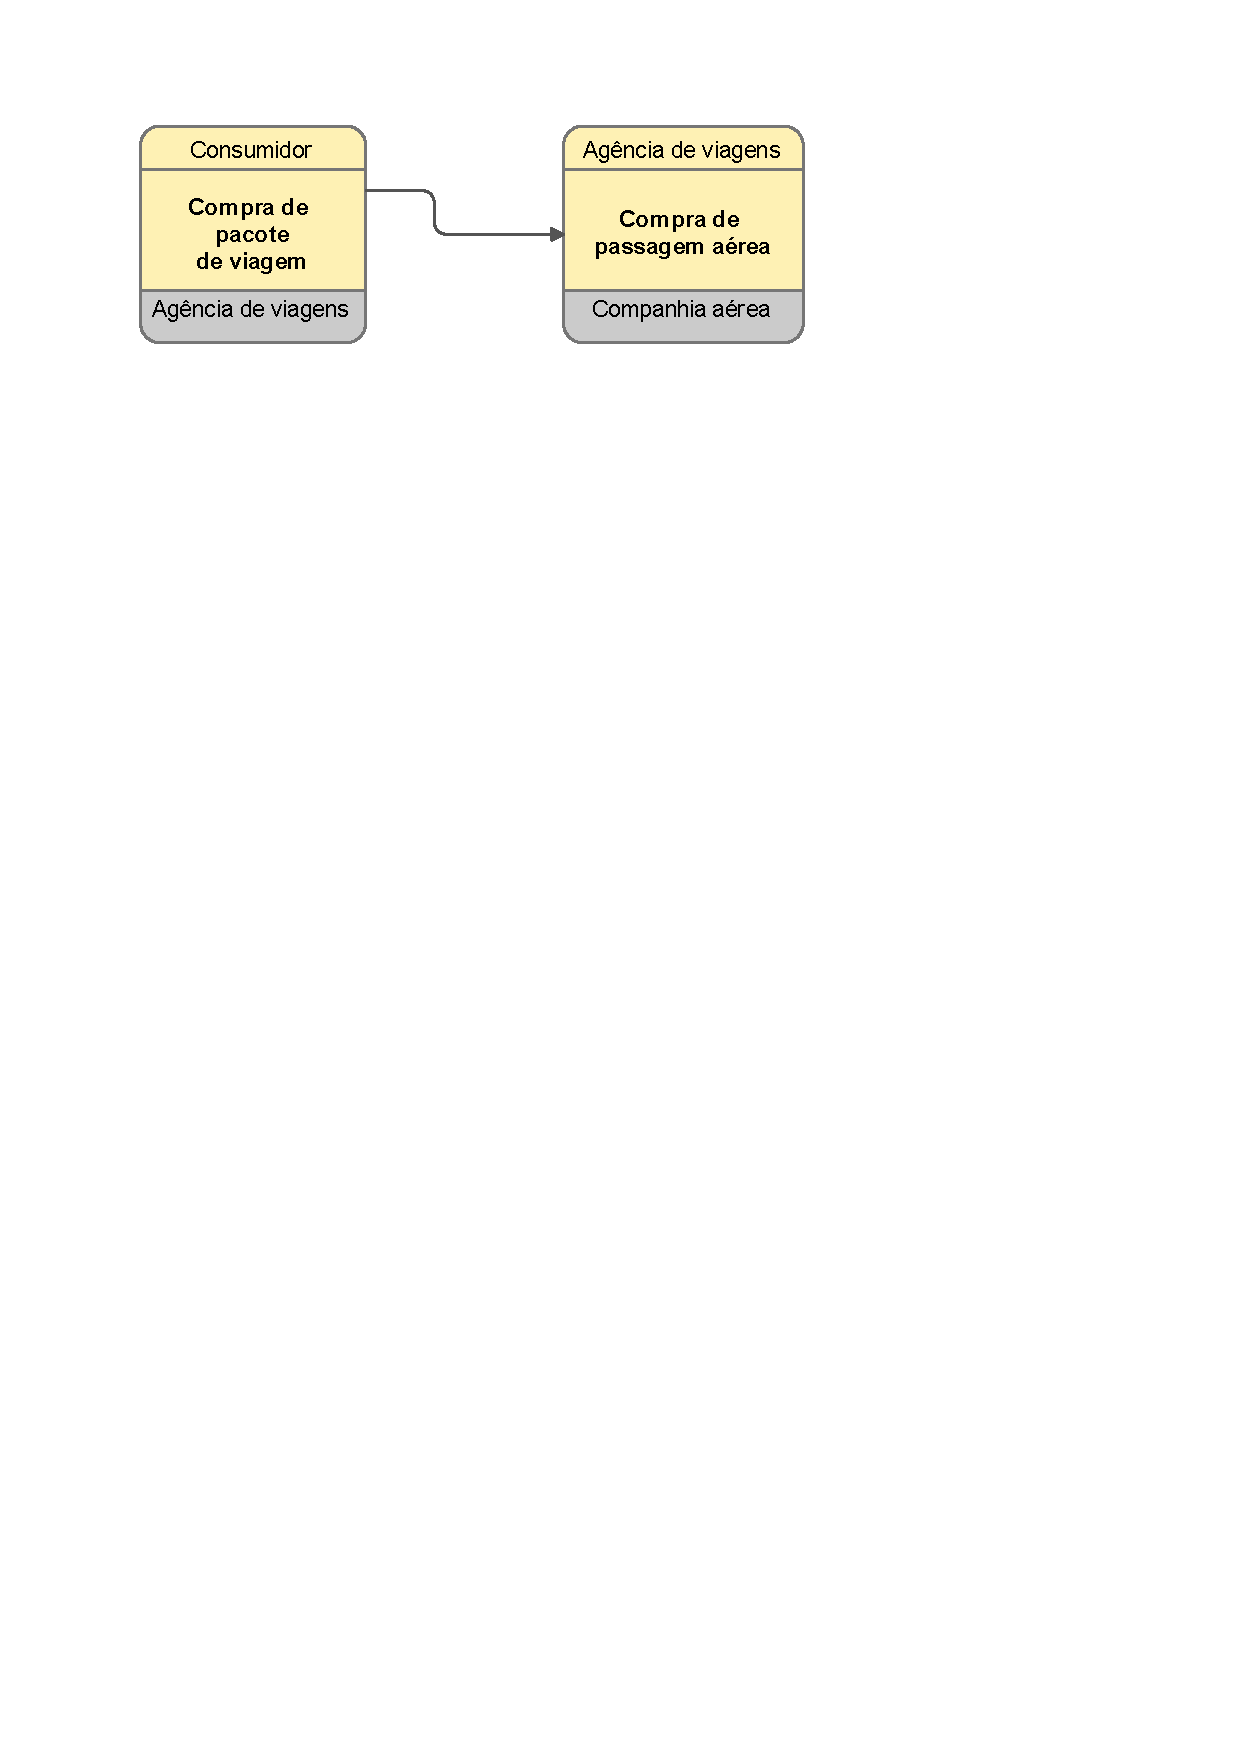
\includegraphics[width=.60\textwidth]{bpmn1.pdf} 
  \caption{Exemplo de uma pequena coreografia de serviços em notação BPMN2}
  \label{fig:bpmn1} 
\end{figure}

Serviços podem ser projetados para participarem de uma determinada composição, mas também é possível que uma composição seja projetada para utilizar serviços já existentes. No segundo caso, é necessária a criação de serviços de coordenação que fazem com que serviços já existentes, não-cientes da composição, comuniquem-se adequadamente~\cite{Autili2013Synthesis}. 

Em artigos acadêmicos também é comum a modelagem de coreografias com notações mais formais, tais como álgebras de processos, redes de Petri e autômatos. Essas notações possibilitam aos autores realizarem simulações e identificarem propriedades, como a verificação da consistência da evolução dinâmica de coreografias~\cite{Cicirelli2010Dynamically}. Em nosso trabalho, como estamos preocupados em viabilizar a execução de coreografias, adotamos como modelagem de referência a notação BPMN2, que é um padrão de indústria.

\section{O processo de implantação de sistemas}
\label{sec:implantacao}

A ``Especificação de implantação e configuração de aplicações distribuídas baseadas em componentes'' (DEPL~\cite{DEPL2006}) é um padrão da OMG (Object Management Group). 
A implantação é definida pelo DEPL como um \emph{processo}, que se inicia após a aquisição de um componente, e vai até o momento em que o componente está em execução, pronto para processar chamadas. 

Embora nosso trabalho foque na implantação de serviços, os conceitos para implantação de componentes também se aplicam à implantação de serviços. 
Mas no contexto de implantação, pode-se dizer que a principal diferença seja o fato de que o \emph{implantador} do serviço seja a própria organização que o desenvolveu, enquanto que o conceito de componentes está mais ligado a um suposto mercado de componentes, em que uns desenvolvem, empacotam e publicam o componente, enquanto que outros adquirem e implantam o componente.

Quando possível, utilizaremos a terminologia estabelecida pelo DEPL em nosso trabalho.
Os principais termos definidos no DEPL e utilizados neste trabalho são os seguintes:

\begin{description}
\item [Implantador:] é a pessoa, ou organização, que é a ``dona'' do componente, e que será responsável pelo processo de implantação. Não é o software que propriamente realiza o processo de implantação.
\item [Ambiente alvo:] a máquina, ou conjunto de máquinas, onde os componentes serão implantados.
\item [Nó:] um recurso computacional onde se implanta um componente, 
como por exemplo uma máquina virtual; faz parte do ambiente alvo.
\item [Pacote:] artefato executável que contém o código binário do componente.
É através do pacote que um serviço pode ser instalado e executado em um determinado
sistema operacional. Existem pacotes dependentes de sistema operacional (ex: deb, rpm),
e pacotes independentes de sistema operacional (ex: jar, war).
\end{description}

Ainda segundo o DEPL, o processo de implantação é composto pelas seguintes fases:

\begin{description}
\item [Instalação:] o implantador transfere o componente adquirido para sua própria infraestrutura; a instalação está relacionada ao processo de aquisição do componente, e não se trata de mover o componente para o ambiente alvo, no qual será executado. Consideramos que essa fase não se aplica à implantação de serviços, pois após o desenvolvimento e empacotamento, o serviço já é de propriedade do implantador e já se encontra em sua infraestrutura.
\item [Configuração:] edição de arquivos de configuração para alterar o comportamento do software; 
o código compilado do componente junto de sua configuração são os insumos para a produção do pacote do componente.
\item [Planejamento:] resulta em um \emph{plano de implantação}, que mapeia como os componentes serão distribuídos pelos nós do ambiente alvo.  
\item [Preparação:] procedimentos no ambiente alvo para preparar a execução do componente. Envolve configurações do sistema operacional, instalação de middlewares (e.g. Tomcat), e a transferência do componente para a máquina onde será executado. 
\item [Inicialização:] é quando finalmente o componente é iniciado e entra em execução, podendo processar chamadas de seus clientes. A inicialização também inclui a ligação entre os componentes de uma composição, para que os componentes conheçam a localização dos componentes dos quais dependem.
\end{description}

Esse processo de implantação pode ter que ser repetido várias vezes para que o componente
seja implantado em todas as etapas do ``\emph{pipeline de implantação}''~\cite{Humble2011Continuous},
como testes de aceitação (automatizados ou não), ambiente de homologação, e finalmente ambiente de produção. 
Todo o processo que vai desde o \emph{commit} do código-fonte,
passando pelas etapas do \emph{pipeline} de implantação, até a implantação em produção
chamaremos de processo de \emph{lançamento} de uma determinada versão do sistema.

Profissionais da acadêmia e da indústria levantam a necessidade de se automatizar o processo de implantação, uma vez que o processo de implantação manual se torna moroso e propenso a erros, principalmente na implantação de sistemas distribuídos~\cite{Humble2011Continuous,Dolstra2005Configuration}. 
Humble e Farley~\cite{Humble2011Continuous} afirmam que o processo de implantação manual faz com que  
o lançamento de uma nova versão do sistema se torne um grande evento nas organizações, 
em que há muita tensão e que faz as pessoas trabalharem até mais tarde.
A solução para esses sintomas, segundo os autores, é a automação do processo de implantação.
Em um processo de implantação automatizado tudo o que for possível é executado de forma automatizada,
geralmente por meio de scripts. O objetivo de um processo de implantação automatizado
é proporcionar um processo de implantação \emph{reproduzível}, \emph{confiável} e \emph{fácil}~\cite{Humble2011Continuous}.

A automação discutida nos trabalhos de Humble, afeta principalmente as fases de preparação e inicialização do modelo de implantação do DEPL. A automação dessas fases normalmente são realizadas com a escrita de scripts, com ou sem ferramentas específicas. Mas há também muitos trabalhos acadêmicos sobre a fase de preparação, envolvendo a escolha automática da máquina alvo de um componente baseado nos requisitos não-funcionais do componente. Por fim, a fase de configuração é menos adequada para se automatizar, pois em geral envolve escolhas que devem ser feitas por humanos (ex: logotipo da empresa, que deve aparecer no cabeçalho do sistema).

Um processo de implantação pode ser automatizado de várias maneiras.
Pode-se utilizar linguagens de script de propósito geral (Python, shell script),
ferramentas gerais voltados para o processo de implantação (ex: 
Chef\footnote{\url{http://www.getchef.com/}}, Capistrano\footnote{\url{https://github.com/capistrano/capistrano}}),
ou middlewares especializados em determinados tipos de artefatos implantáveis,
entre os quais se enquadram as soluções de Plataforma como um Serviço,
sobre as quais discutiremos na Seção~\ref{sec:cloud}.
Humble e Farley recomendam a utilização de sistemas especializados, preterindo 
a utilização de linguagens de scripts de propósito geral.

A concretização de um processo de implantação automatizado depende bastante da
integração de diferentes papeis em uma organização, principalmente o dos desenvolvedores
com os operadores, uma vez que o desenvolvimento dos scripts de implantação requer
habilidades de ambos os perfis.
Essa percepção levou à criação do conceito de uma cultura 
rotulada como DevOps~\cite{Humble2011DevOps}, na qual times inter-funcionais
trabalham para a concretização da implantação automatizada.

A discussão a seguir sobre as vantagens do processo de implantação automatizado
são baseadas no livro ``\emph{Continuous Delivery}''~\cite{Humble2011Continuous}.

Muitos problemas na implantação manual se dão por causa de documentação incompleta,
contendo pressupostos não compartilhados por todo o time responsável por um produto ou serviço.
Dessa forma é comum que a organização fique bastante dependente de uma única
pessoa para realizar a tarefa de implantação.
Por outro lado, um script de implantação é uma documentação completa de todos os passos
do processo e que mais dificilmente ficará defasada,
pois nesse caso deixará de funcionar e a implantação não será possível.

A facilidade de se implantar o sistema com o simples pressionar de um botão
leva a sua utilização contínua por diferentes atores.
O time de desenvolvimento estará constantemente utilizando esse script 
para realizar testes de integração e aceitação. 
Essa execução contínua do processo de implantação nos testes trará os seguintes benefícios:

\begin{itemize}
\item Os testes se tornam mais confiáveis por serem executados em um ambiente garantidamente similar ao ambiente de produção.
\item A quantidade de execuções de testes de integração e aceitação será maior, o que auxilia na garantia de qualidade do sistema.
\item O próprio processo de implantação se torna mais confiável, pois quando o ``grande dia'' da implantação chega, o processo já terá sido executado várias vezes.
\item Em particular, é de se esperar que defeitos no script de implantação já tenham sido detectados e corrigidos.
\end{itemize}

A utilização da implantação automatizada na execução de testes também
facilita a execução concorrente de múltiplos testes em ambientes isolados.
Isso, por sua vez, contribui para o aumento da bateria de testes, fazendo com que
a cobertura dos testes aumente e, por fim, a própria qualidade do sistema testado também melhore.

Outro problema na implantação manual é que quando o sistema finalmente é testado
no ambiente de produção, grandes mudanças arquiteturais podem ser economicamente inviáveis.
A implantação automatizada favorece a prática da implantação contínua desde as versões
embrionárias do sistema, ajudando a garantir que decisões arquiteturais são adequadas
e evitando alterações de última hora para adequar o sistema ao ambiente de produção.

A implantação contínua e confiável do sistema é um fator determinante de apoio ao lançamento
contínuo de novas versões. Isso é importante para que se consiga o \emph{feedback} do cliente
o quanto antes sobre as últimas alterações no sistema.
Esse \emph{feedback} é importante tanto do ponto de vista técnico para o aprimoramento do sistema,
quanto do ponto de vista de negócio, pois é ele que ajuda o time a saber se está construindo
\emph{a coisa certa}.
O encurtamento do tempo entre desenvolvimento e \emph{feedback} do cliente
é uma prática pregada pelo movimento da \emph{lean startup}~\cite{Ries2011Lean}.

Na próxima seção falaremos sobre a computação em nuvem,
moderna tecnologia que impacta altamente as técnicas de implantação de sistemas.

\section{Computação em nuvem}
\label{sec:cloud}

O Instituto Nacional de Padrões e Tecnologias dos Estados Unidos (NIST) define computação em nuvem como um ``modelo para possibilitar acesso ubíquo, conveniente e sob demanda pela rede a um conjunto compartilhado de recursos computacionais (por exemplo: redes, servidores, discos, aplicações e serviços) que possam ser rapidamente provisionados e liberados com o mínimo de esforço gerencial ou interação com o provedor do serviço''~\cite{Nist2011Cloud}. 

Zhang et al.~\cite{Zhang2010Cloud} destacam as seguintes características da computação em nuvem: i) separação de responsabilidades entre o dono da infraestrutura de nuvem e o dono do serviço implantado na nuvem; ii) compartilhamento de recursos (serviços de diferentes organizações hospedados na mesma máquina, por exemplo); iii) geodistribuição e acesso aos recursos pela Internet; iv) orientação a serviço como modelo de negócio; v) provisionamento dinâmico de recursos; vi) cobrança baseada no uso de recursos, de forma análoga à conta de eletricidade.

Os serviços de computação em nuvem poder ser oferecidos a clientes internos ou externos à organização administradora da plataforma de nuvem. Quando os clientes são externos dizemos que a nuvem é pública, como no caso da nuvem da Amazon; quando os clientes são internos, dizemos que a nuvem é privada, situação na qual a organização pode utilizar ambientes baseados em um middleware como o OpenStack~\cite{Zhang2010Cloud}.

À computação em nuvem é atribuída os seguintes modelos de negócio~\cite{Zhang2010Cloud}, ou modelos de serviço~\cite{Nist2011Cloud}: Infraestrutura como um Serviço (IaaS), Plataforma como um Serviço (PaaS) e Software como um Serviço (SaaS). 

O modelo de Infraestrutura como Serviço (IaaS) fornece acesso aos recursos virtualizados, como máquinas virtuais, de forma programática. Um dos principais fornecedores atuais de IaaS é a Amazon, com os serviços Amazon Web Services (AWS). Dentre os vários serviços fornecidos pela plataforma, destaca-se o EC2, que possibilita a criação e gerenciamento de máquinas virtuais na nuvem da Amazon. Na utilização de IaaS, uma das considerações chaves é ``tratar hospedeiros como efêmeros e dinâmicos''~\cite{Amazon2012Practices}. É preciso considerar que hospedeiros podem ficar indisponíveis e que nenhuma suposição pode ser feita sobre seus endereços IPs, o que requer um modelo de configuração flexível e que a inicialização do hospedeiro leve em conta essa natureza dinâmica da nuvem. Para que as aplicações sejam escaláveis e tolerantes a falhas, a Amazon recomenda mais do que a criação de máquinas virtuais com o serviço EC2: deve-se utilizar grupos de máquinas replicadas que compartilhem um balanceador de carga~\cite{Amazon2012Practices}. Conforme a demanda da aplicação cresce ou diminui, máquinas podem ser dinamicamente acrescentadas ou removidas desses grupos de replicação, o que proporciona escalabilidade horizontal à aplicação. Naturalmente, essa replicação depende de um prévio preparo da aplicação para esse cenário, pois se deve levar em conta a distribuição, replicação e particionamento dos dados. 

O uso de recursos virtualizados, proporcionado pelo modelo IaaS,
potencializa a automação do processo de implantação~\cite{Humble2011Continuous}.
Novos ambientes podem ser criados dinamicamente, em poucos minutos,
com a configuração de um sistema operacional recém instalado em uma máquina.
Isso traz as seguintes vantagens para o processo de implantação:

\begin{itemize}
\item Evita-se a burocracia e custos necessários para o provisionamento de novo hardware.
\item A implantação pode ser repetida facilmente no mesmo ambiente, não é preciso reinstalar o sistema operacional ou limpar as configurações do sistema para se obter uma nova implantação do serviço.
\item Se executados em diferentes máquinas virtuais, dois serviços podem dividir um mesmo servidor físico sem que a implantação e execução de um serviço afete a execução do outro serviço anteriormente implantado.
\end{itemize}

Na utilização de serviços IaaS para a implantação de serviços há duas abordagens possíveis:
1) a máquina virtual deve ser criada com base em uma imagem que já contenha
o serviço implantado, ou 2) deve ser criada com base em uma imagem contendo apenas um
sistema operacional recém instalado, de forma que a implantação do serviço seja feita
por scripts. O modelo de imagem pronta pode proporcionar implantações mais rápidas,
porém a segunda abordagem é mais flexível e ágil, pois evita-se a manutenção constante
das imagens. Um compromisso entre as duas abordagens também é possível:
se todos os serviços implantados são WARs, por exemplo, então a imagem base
pode conter não só o sistema operacional, mas também o ambiente de execução
dos serviços, o Tomcat no caso.

No modelo de Plataforma como Serviço (PaaS) os desenvolvedores da aplicação não precisam preocupar-se diretamente com a gerência dos recursos virtualizados ou com a configuração dos ambientes nos quais a aplicação será implantada, concentrando-se no desenvolvimento do código da aplicação.
Um exemplo típico de PaaS é o Google App Engine\footnote{\url{https://developers.google.com/appengine/}}, que oferece implantação transparente a projetos em Python, Java ou Go. O App Engine também oferece escalabilidade automática de modo mais simples que os serviços de IaaS, uma vez que a configuração prévia e as alterações na infraestrutura ocorrem de modo totalmente transparente ao desenvolvedor da aplicação. Uma desvantagem presente nos serviços PaaS são as restrições de linguagens, bibliotecas e ambientes impostas aos desenvolvedores da aplicação.

Como exemplo de SaaS temos o Google Docs ou qualquer outro aplicativo online que seja diretamente utilizado pelo usuário final. Uma das aplicações desse tipo é o armazenamento de dados na nuvem, como fornecido pelo Dropbox\footnote{\url{http://dropbox.com/}}. Uma confusão comum é definir o conceito de nuvem como se fosse estritamente ligado a esse tipo de serviço de armazenamento de dados.

Com as vantagens aqui apresentadas, é cada vez mais comum o uso dos recursos de nuvem por empresas que desenvolvem software, pois assim seus esforços concentram-se no desenvolvimento do produto, aliviando as preocupações com infraestrutura. A computação em nuvem também possibilita que organizações evitem grandes investimentos antecipados em infraestrutura, pois os recursos virtualizados são dinamicamente acrescentados conforme a carga da aplicação requeira. Pode-se então considerar o uso da nuvem uma realidade do mercado de software atual. Dessa forma, é natural esperar que a implantação de composições de serviços também se dê no ambiente de computação em nuvem, que é a abordagem deste trabalho. 

\section{Desafios na implantação de sistemas de grande escala}

Na visão proposta pelo Instituto de Engenharia de Software da Universidade Carnegie Mellon, sistemas de ultra grande escala serão ultra grandes em relação a todas as dimensões possíveis: linhas de código, pessoas, dados, dispositivos, etc.~\cite{CarnegieMellon2006ULS}. O número estimado de linhas de código desses sistemas é de bilhões. Para efeito de comparação, o núcleo do sistema operacional GNU/Linux possui cerca de 15 milhões de linhas de código em sua versão 3.2, a mais recente no momento da escrita deste texto~\cite{Leemhuis2012Statistics}. Com isso, talvez o único sistema da atualidade que se assemelha aos sistemas de escala ultra grande previstos é a Internet. 

A característica mais importante de um sistema de grande escala não é seu tamanho, mas o fato de ser caracterizado como um ``ecossistema sociotécnico''~\cite{CarnegieMellon2006ULS}, em que pessoas são parte integrante do sistema, interagindo com diferentes objetivos, de modo decentralizado e independente, porém seguindo restrições impostas. A analogia proposta é de que o desenvolvimento dos atuais sistemas de grande escala equipara-se a construção de prédios, enquanto que o desenvolvimento de sistemas de escala ultra grande equivaleriam a construção de cidades, o que é naturalmente um processo contínuo e decentralizado.

Recentemente temos ainda a consolidação da computação em nuvem, que traz um conjunto de tecnologias e práticas que se relacionam com as três características de sistemas de escala ultra grande anteriormente mencionadas. Sistemas distribuídos estão migrando para ambientes de nuvem, onde são compostos e mantidos decentralizadamente por várias organizações~\cite{Steen2011VeryLarge}. A virtualização, um dos aspectos centrais da computação em nuvem, é de grande auxílio no provisionamento de novos ambientes~\cite{Humble2011Continuous}, o que é importante para o processo de implantação de sistemas. A virtualização também facilita a criação de ambientes replicados, arquitetura importante para tratar falhas individuais de componentes.

A grande escala afeta os processos envolvidos no ciclo de vida dos sistemas.
Estudando a literatura que aborda e discute desafios, princípios e práticas de
sistemas de grande escala, identificamos os seguintes desafios que essa nova
realidade traz ao processo de implantação de sistemas:

\begin{description}

\item [Processo:]

Como já foi discutido neste capítulo, a automação do processo de implantação
vem se firmando como uma tendência crucial na capacidade
das equipes de TI entregarem valor o mais continuamente possível,
evitando as dificuldades e problemas presentes no processo manual de implantação.
Tais dificuldade e problemas se tornam muito mais complicados em ambientes distribuídos
e de grande escala. Por isso, nesse caso a automação dos processos se torna
ainda mais fundamental.
Hamilton~\cite{Hamilton2007InternetScale} lista uma série de boas práticas acumuladas 
por anos de experiência no desenvolvimento de serviços de grande escala.
Dentre elas, Hamilton destaca a automação de todos os processos de operações dos serviços,
alegando que processos automatizados são testáveis, reparáveis e, portanto,
mais confiáveis.

\todo{rollback}

\todo{idempotência (Chef valoriza isso no processo de implantação)}

\item [Falhas de terceiros:] 

Sistemas distribuídos de grande escala devem esperar e tratar falhas
de componentes de terceiros~\cite{Hamilton2007InternetScale,Helland2009Quicksand,CarnegieMellon2006ULS}.
Mesmo se a chance de falhas de cada componente é pequena,
a grande quantidade de componentes e interações aumenta as chances de 
falhas em algum lugar do sistema~\cite{CarnegieMellon2006ULS}.
Mais do que ser projetado para não falhar, um componente operando em um ambiente  de grande escala deve ser projetado para tratar adequadamente situações de exceção e indisponibilidade, tanto do próprio componente, quanto de outros componentes dos quais depende.

Um exemplo de falha típica em um processo de implantação automatizado
utilizando um serviço de IaaS envolve o provisionamento de VMs.
Quando um novo nó é requisitado para o provedor de infraestrutura,
há uma chance de que o provisionamento falhe.
Além disso, alguns nós podem levar um tempo muito maior que a média para ficarem prontos.
Outras operações que podem falhar durante o processo de implantação são
conexões SSH e a execução de scripts nos nós alvos.

A Figura~\ref{fig:ec2_boxplot} mostra a distribuição por nós observada
do tempo de criação de VMs quando se requisita concorrentemente a criação
de 100 nós na nuvem da Amazon (isso foi repetido 10 vezes).
Nós contamos o tempo que vai da requisição de criação do nó
até o momento em que a VM se encontra apta a receber conexões SSH,
que é quando ela se torna pronta para uso na prática.
Nós observamos uma taxa de falha de 0.6\%
quando se tenta criar concorrentemente 100 nós.
É interessante notar que o tempo de criação tem uma mediana estável,
mas que alguns valores altos para esse tempo são esperados quando
se cria ao mesmo tempo uma grande quantidade de nós.
Em nossas observações, falhas e tempos longos de provisionamento
afetaram até 7\% das requisições de criação de nós.

\begin{figure}[ht]
\centering
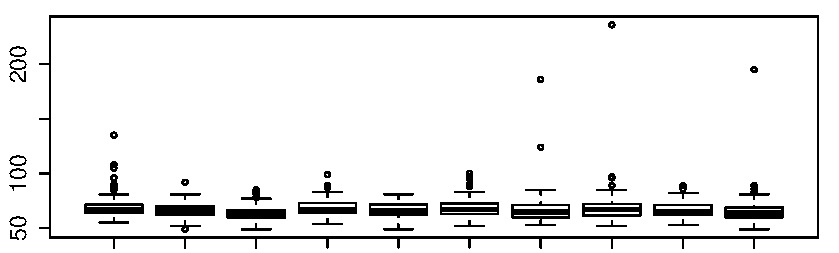
\includegraphics[width=\linewidth]{ec2_boxplot.pdf}
\caption{Tempos de criação de instâncias EC2 observados, em segundos.}
\label{fig:ec2_boxplot}
\end{figure}

\item [Disponibilidade:]

Embora serviços em um sistema distribuído tenham que estar preparados para lidar
com a falha de outros serviços do sistema,
cada serviço deve ter sua disponibilidade aumentada tanto quanto possível. 
Para isso é preciso aplicar técnicas que
aumentem o tempo médio entre falhas e/ou diminuam o tempo médio de reparo após uma falha.

O balanceamento de carga entre réplicas de um serviço é uma das práticas mais importantes e 
recomendados atualmente para aumentar a disponibilidade e escalabilidade de sistemas~\cite{Amazon2012Practices}.
Com a replicação do serviço, a falha em uma réplica não implica na indisponibilidade
do serviço. Além disso, com a utilização das tecnologias de nuvem,
caso a quantidade de requisições aumente, pode-se requisitar um aumento na quantidade de réplicas,
o que evitará uma indisponibilidade por incapacidade de se atender a todas as requisições.

Outra prática importante para o aumento da disponibilidade é a replicação de dados~\cite{Brewer2001GiantScale}.
No entanto, a replicação síncrona de dados é inviável para sistemas de grande escala~\cite{Helland2009Quicksand}.
O Teorema CAP~\cite{Brewer2012Cap} prevê que um sistema não mantém os níveis de consistência e de disponibilidade na presença de particionamentos de rede. Considerando que particionamentos de rede são intrínsecos ao ambiente da Internet, o aumento no tamanho dos sistemas inviabilizou uma consistência total com tempo de resposta satisfatório. 
Essa mudança representou uma quebra de paradigma na área de bancos de dados,
pois agora os bancos de dados projetados para fornecer as propriedades ACID,
que garantem consistência total, cedem lugar aos cada vez mais populares
bancos de dados não-relacionais (NoSQL).
Essa nova categoria sacrifica a consistência dos dados para obter maior disponibilidade ou escalabilidade~\cite{Cattell2011NoSql}.

O processo de implantação deve considerar as necessidades de replicação de serviços e dados,
para que possa configurar adequadamente as múltiplas instâncias dos serviços e das bases de dados.
Deve ser possível também alterar em tempo de execução a quantidade de réplicas para
a adequação à demanda observada.

\item [Escalabilidade:]

Quando se implanta uma grande quantidade de serviços em um ambiente distribuído,
não é desejável que as implantações dos diferentes serviços sejam sequenciais.
Uma vez que a implantação de diferentes serviços são tarefas independentes,
implanta-los concorrentemente aumenta drasticamente a escalabilidade
do processo de implantação da composição.

Dizemos que uma arquitetura é perfeitamente escalável
se ela continua a apresentar o mesmo desempenho por recurso,
mesmo que usado em um problema de tamanho maior, conforme o número
de recursos aumenta~\cite{Quinn1994Scalability}.
No contexto de implantação, isso significa que, idealmente,
o tempo de implantação deveria permanecer constante quando há um
aumento proporcional no número de serviços a serem implantados e
no número de nós alvos.

Note que o número de serviços a ser implantado aumenta em duas situações:
1) quando se implanta composições maiores e 2) quando se implanta
mais composições simultaneamente. 
A primeira situação ocorre na implantação de sistemas de grande escala.
A segunda situação pode ocorrer, por exemplo,
quando se executa uma bateria de testes de aceitação de uma composição de serviços.
Note que nesse caso um teste de aceitação pode levar um tempo considerável,
já que engloba o provisionamento de um novo nó e a preparação do sistema.
Em tal situação, é desejável que testes de aceitação sejam executados em paralelo,
o que requer implantação concorrente de múltiplas instâncias da mesma composição.
Quanto maior a capacidade de paralelização desse processo,
mais testes poderão ser admitidos na bateria de testes.

\item [Heterogeneidade:]

Componentes de sistemas de grande escala normalmente são construídos com diferentes tecnologias
e hospedados em diferentes tipos de ambientes.
Um dos principais caminhos para viabilizar a coexistência dessa pletora tecnológica
é a Arquitetura Orientada a Serviços, incluindo as composições de serviços web.

Embora serviços web tenha surgido para resolver os problemas de heterogeneidade
entre sistemas e organizações, hoje em dia temos mais de um mecanismo para
implementar o conceito serviços, principalmente SOAP e REST, além de outros.
Portanto, suportar heterogeneidade é importante para sistemas baseados em serviços.
A falta de flexibilidade para a escolha de tecnologia para o desenvolvimento de serviços
e o provedor de infraestrutura ocorre em muitas soluções PaaS atualmente disponíveis.

\item [Múltiplas organizações:]

Sistemas de grande escala não possuem um único dono~\cite{Steen2011VeryLarge}, 
sendo que seus componentes pertencem a diferentes organizações que interagem de forma coordenada. 
O conceito de coreografias de serviços web e notações como o BPMN surgem para 
formalizar a interação entre serviços de organizações diferentes em tempo de execução.

Em uma composição inter-organizacional a coordenação do processo de implantação se torna um desafio. Normalmente não se admite que um coordenador em uma organização possa tomar decisões 
sobre a implantação de serviços de outra organização, pois esse processo envolve
custos, acesso a infraestrutura e acesso ao pacote do serviço.
Dessa forma, não podemos esperar que haja um orquestrador para coordenar o processo de implantação.
As organizações deveriam agir de forma colaborativa para que o processo de implantação
da composição tenha sucesso.
No entanto isso não é tão simples, pois no caso de implantação simultânea,
é preciso haver algum protocolo de comunicação para que uma organização receba
por notificação os endereços de serviços recém implantados por outra organização,
quando esses serviços são dependências de seus próprios serviços sendo também implantados.

\item [Adaptabilidade:]

\end{description}



